% Section for the report: Hypothesis 1 (Shakespeare-char language modelling).
% Needs: \usepackage{graphicx,booktabs,amsmath}.  Figure/table files are in report/h1/ (upload them next to the .tex):
%   fig_h1_curves.pdf  fig_h1_final.pdf  fig_h1_tune.pdf  table_h1.tex
% Citation keys below are placeholders: replace shumaylov / jordan / loshchilov with your bib keys
% (the draft's [4] = Shumaylov et al., [5] = Jordan et al., [1] = Loshchilov & Hutter).
% The paper calls the random-spectrum optimizer "Kaon" (the spec writes "Keon"); this text uses Kaon.

\section{Language modeling - H1 (David)}

\subsection{Setup}

\paragraph{Model and data:}
We train a nanoGPT-style decoder-only transformer with 6 layers, 6 heads and width $d_{\text{model}}=384$
(10.73M parameters): pre-LayerNorm blocks, GELU MLPs with a $4\times$ hidden width, no biases, tied input/output embeddings, dropout $0.2$ and a
context of 256 tokens. The data is the character-level Tiny Shakespeare corpus (vocabulary of 65 characters;
1{,}003{,}854 training and 111{,}540 validation characters). Each step uses a batch of $64\times256$ tokens, so the
5000 steps of a run correspond to about 80 passes over the training text. The 24 hidden matrices
(fused QKV, attention output, and the two MLP matrices in each of the 6 blocks) are updated by the optimizer under
test. Embeddings, positional embeddings and LayerNorm parameters are always updated by AdamW
whatever the spectral optimizer, at the ``base'' learning rate $\eta_B$ that \cite{shumaylov} tune alongside the matrix learning rate $\eta_M$.
The paper does not state the remaining AdamW settings; we use the nanoGPT defaults ($\beta=(0.9,0.95)$, weight decay $0.1$ on the embeddings and none on the LayerNorm parameters) and no gradient clipping.

\paragraph{Optimizers:}
Let $G=U\Sigma V^\top$ be the momentum-averaged gradient of a hidden matrix. Every spectral optimizer replaces $G$ by a matrix with the same singular vectors and a
different spectrum:
\begin{itemize}
  \item \textbf{Muon:} five steps of Jordan's quintic Newton--Schulz iteration~\cite{jordan}, which drives all singular values of $G$ towards a band around $1$.
  \item \textbf{Freon} (exponent $c$): $(GG^\top)^{-c}G=U\Sigma^{1-2c}V^\top$, normalised by the power mean $\mu=(\tfrac1r\sum_i\sigma_i^{q})^{1/q}$ with $q=2(1-c)$, as in App.~H.3 of~\cite{shumaylov}.
        $c=0$ is SGD, $c=\tfrac12$ is the exact polar factor (Muon's ideal), and for $c>\tfrac12$ the spectrum is \emph{inverted}: small singular directions are amplified. We run $c=2/3$ and $c=3/4$.
        \textbf{We compute this exactly} through a float64 eigendecomposition of $GG^\top$ (a float64 SVD is numerically equivalent, checked in our tests), \emph{not} with the paper's
        approximate QDWH iteration.
  \item \textbf{Kaon:} no spectral structure is kept: $X_0=G/\|G\|_F$, five steps of $X\leftarrow 4.1\,(I-XX^\top)^2X$ (Alg.~2 of~\cite{shumaylov}), then division by $1.175$. The singular values of the result are
        a fixed, chaotic function of the normalised input singular values.
  \item \textbf{TruncatedSGD:} zero the top $\lceil 0.05\,r\rceil$ singular values of $G$ and rescale to $\|G\|_F$, $r=\operatorname{rank}$.
  \item \textbf{SGD:} the unmodified momentum update on the same matrices.
\end{itemize}

\paragraph{Training details:}
Spectral methods use Nesterov momentum $0.95$ and the Muon shape factor $\sqrt{\max(1,m/n)}$ for an $m\times n$ matrix; SGD and TruncatedSGD use momentum $0.9$ and no shape factor, following~\cite{shumaylov}.
All runs use 5000 steps, a 100-step linear warmup, and cosine decay to $10\%$ of the peak learning rate, in bf16 autocast on one NVIDIA L4. Validation loss is evaluated every 250 steps on 50 fixed batches.
We tune the matrix learning rate $\eta_M$ and the AdamW learning rate $\eta_B$ separately per optimizer (Appendix, Fig.~\ref{fig:h1tune}):
\emph{(1) Tune:} seed 42, 1500 steps per run. Muon and Kaon were first run on the 16-point grid of \cite{shumaylov}; since their best point lay on the edge of it
($\eta_M=0.02$) we extended it with $\eta_M=0.04$ and $\eta_B=5\!\times\!10^{-4}$. Freon used a focused grid $\eta_M\in\{0.01,0.02,0.04\}\times\eta_B\in\{5\!\times\!10^{-4},10^{-3},2\!\times\!10^{-3}\}$ (9 points).
SGD and TruncatedSGD act on the raw gradient and need much larger steps, so they use their own grid ($\eta_M$ up to $10$, $\eta_B$ up to $4\times10^{-3}$).
This is 83 tuning runs. \emph{(2) Final:} the best point of each optimizer is re-run for 5000 steps with seeds 42, 43, 44 (18 runs).
We report the \emph{best} validation loss seen during training (the metric of H1), and also the final loss.
As in the rest of this report, ``within seed noise'' means a difference smaller than one sample standard deviation across seeds.

\subsection{Results}

Overall, the main claim of~\cite{shumaylov} reproduces at this scale. Muon, Freon at $c=2/3$ and $c=3/4$, and Kaon reach the same best validation loss (Table~\ref{tab:h1main}, Fig.~\ref{fig:h1final}), even though Freon inverts the spectrum and Kaon has no
spectral structure. TruncatedSGD is clearly worse, and plain SGD is behind but within the spread of its own seeds.

\begin{table}[t]
  \centering
  \caption{Hypothesis 1, Shakespeare-char: validation loss (mean $\pm$ sample std over seeds 42/43/44) at the tuned learning rates, 5000 steps. ``Best'' is the lowest validation loss during training, ``final'' the loss at step 5000.
  $\Delta$ is the mean best-loss gap to Muon and $p$ a Welch $t$-test against Muon on the best loss (3 seeds each, so low power). Time is the wall-clock of one 5000-step run on an L4 (Freon: eigendecomposition implementation).}
  \label{tab:h1main}
  \resizebox{\textwidth}{!}{\begin{tabular}{lrrrrrrr}
\toprule
Optimizer & $\eta_M$ & $\eta_B$ & Best val loss & $\Delta$ vs Muon & Welch $p$ & Final val loss & Time (min) \\
\midrule
Muon & 0.02 & 0.001 & $\mathbf{1.4438 \pm 0.0053}$ & - & - & $1.5355 \pm 0.0043$ & 5.2 \\
Freon $c=2/3$ & 0.02 & 0.001 & $1.4449 \pm 0.0031$ & +0.0010 & 0.79 & $1.4991 \pm 0.0052$ & 19.4 \\
Freon $c=3/4$ & 0.02 & 0.001 & $1.4479 \pm 0.0056$ & +0.0041 & 0.41 & $1.4912 \pm 0.0087$ & 19.4 \\
Kaon & 0.04 & 0.002 & $1.4480 \pm 0.0057$ & +0.0042 & 0.40 & $1.5568 \pm 0.0064$ & 5.0 \\
\midrule
TruncSGD 5\% & 10 & 0.004 & $1.4875 \pm 0.0015$ & +0.0436 & <0.01 & $1.4875 \pm 0.0015$ & 35.6 \\
SGD & 10 & 0.002 & $1.4716 \pm 0.0222$ & +0.0277 & 0.16 & $1.4819 \pm 0.0155$ & 4.6 \\
\bottomrule
\end{tabular}
}
\end{table}

\begin{figure}[t]
  \centering
  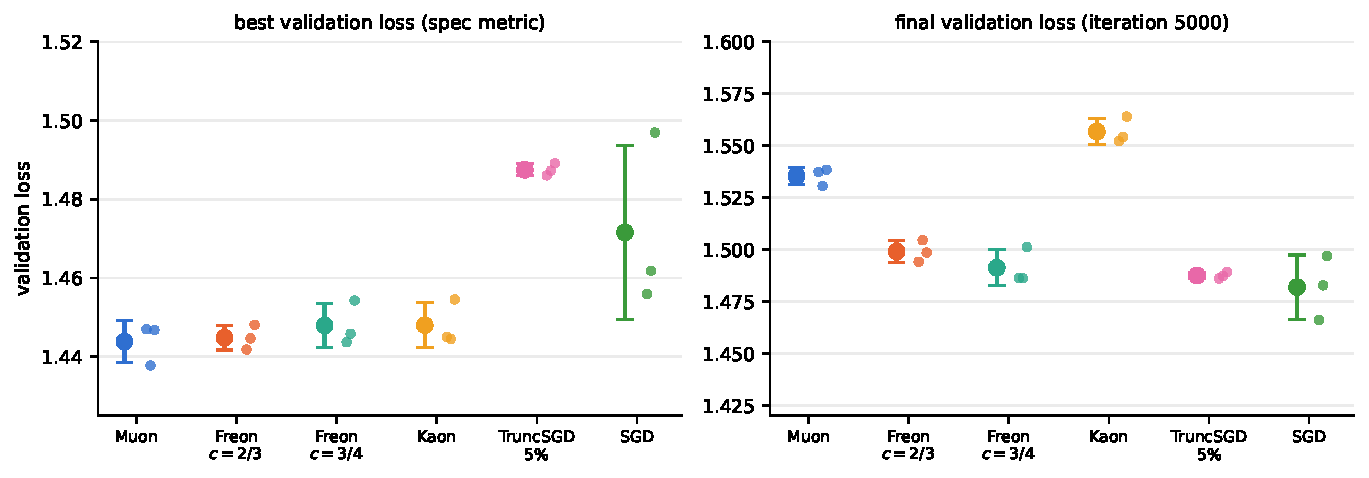
\includegraphics[width=\textwidth]{fig_h1_final.pdf}
  \caption{Per-seed validation loss. The large marker and bar are the mean $\pm$ one sample std, the small dots to its right are the three seeds. Left: best validation loss. Right: loss at step 5000.
  Muon, both Freons and Kaon are indistinguishable on the best loss; the ranking on the final loss is reversed because of overfitting (see text).}
  \label{fig:h1final}
\end{figure}

\paragraph{Performance of Muon, Freon and Kaon:}
The four methods end within $0.0042$ of each other (best loss $1.4438$ to $1.4480$), which is smaller than the seed std of Muon ($0.0053$). Freon at $c=2/3$ is $0.0010$ above Muon ($p=0.79$), Freon at $c=3/4$ is
$0.0041$ above ($p=0.41$) and Kaon $0.0042$ above ($p=0.40$). So Freon with the quasi-norm exponent $c=2/3$ and the chaotic Kaon map both match Muon, which is the headline claim of the paper and our H1.
The paper scans more values of $c$; we only ran $c=2/3$ and $c=3/4$, so we cannot say where the optimum lies. We note that $c=3/4$ is slightly (not significantly) worse than $c=2/3$, in the same direction as the CIFAR-10 result of Section~2.

\begin{figure}[t]
  \centering
  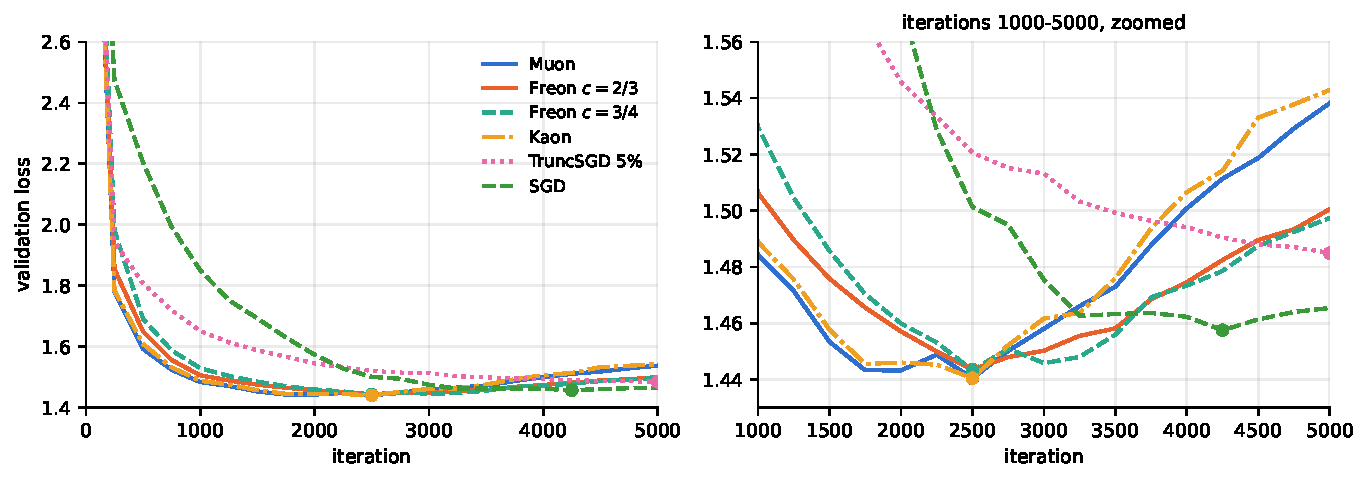
\includegraphics[width=\textwidth]{fig_h1_curves.pdf}
  \caption{Validation loss during training (seed 42); dots mark each run's best loss. Right: zoom on steps 1000--5000. Muon, Kaon and both Freons descend together and reach their minimum at about step 2500 ($1.4405$--$1.4436$), then overfit.
  SGD and TruncatedSGD are far behind early and are still improving, or have only just stopped improving, at the end of training.}
  \label{fig:h1curves}
\end{figure}

The curves (Fig.~\ref{fig:h1curves}, one seed) show how the methods get there. The four flattening/random methods are nearly on top of each other for the whole run: they reach about $1.48$--$1.53$ after 1000 steps and all
reach their best loss at around step 2500. After that every one of them overfits (the model sees each training character about 40 times by then), so the loss at step 5000 is higher than the best one:
$1.536$ for Muon and $1.557$ for Kaon. The two Freon variants overfit less ($1.499$ and $1.491$), so on the \emph{final} loss they are ahead of Muon and Kaon, a ranking opposite to the best loss. We therefore read the final-loss column as a measure of overfitting
speed, not of optimizer quality, and use the best loss for H1. In steps the four methods are equally fast; they differ in cost per step: with our exact eigendecomposition, Freon takes $19.4$ minutes per run against $5.2$ for Muon and $5.0$ for Kaon.
This overhead comes from our implementation (the paper's QDWH iteration is built from matrix multiplications), so the cost column should not be read as an intrinsic property of Freon.

\paragraph{SGD and Truncated SGD:}
Both baselines are behind Muon on the best loss, TruncatedSGD clearly and SGD within noise. TruncatedSGD ends at $1.4875\pm0.0015$, $0.044$ above Muon ($p<0.01$; the seeds agree to within $0.003$), and it is still decreasing at step 5000, so it has not even reached a minimum.
SGD ends at $1.4716\pm0.0222$, $0.028$ above Muon, but one of its three seeds is much worse than the others, so with three seeds the gap is not significant ($p=0.16$; the gap is only $1.2$ times SGD's own seed std). The picture
is therefore: \emph{TruncatedSGD lags, SGD lags in the same direction but we cannot call it beyond noise.}
The curves show that SGD's problem is mostly speed: at step 1000 its validation loss is about $1.85$ against $1.48$ for Muon, and at step 2500 $1.50$ against $1.44$; it catches up late (best at step 4250 for seed 42, $1.4575$) and, because it overfits much less, it has the lowest \emph{final} loss of all
methods ($1.482$). In the compute budget of a 5000-step run, the flattening methods are therefore the more efficient choice, but SGD is not far from their best loss once it has trained long enough.
Removing the top $5\%$ of the spectrum (TruncatedSGD) speeds up the start relative to SGD ($1.65$ against $1.85$ at step 1000) but its best loss is not better than SGD's ($1.4875$ against $1.4716$, within SGD's seed spread).
In the tuning grids (Fig.~\ref{fig:h1tune}), the best learning rates of both baselines lie at or next to the largest values we tried ($\eta_M=10$; for TruncatedSGD also $\eta_B=4\times10^{-3}$), so they may be slightly under-tuned.

\paragraph{Caveats:}
(i) Three seeds, so the Welch tests are a guide and not a proof. (ii) Learning rates were tuned at 1500 steps and used at 5000, and tuning seed 42 is also one of the three final seeds (this favours every optimizer equally).
(iii) The learning-curve figure is a single seed (42), not an average. (iv) The language model overfits after $\approx2500$ steps on this small corpus, so the best loss is an early-stopped number; weight decay on the hidden matrices (currently $0$) or a smaller number of steps could change the final-loss ranking.
(v) Our Freon is the exact map and not the paper's approximate QDWH iteration; we did not measure the effect of this on training, and it could in principle go either way.

\paragraph{Code:}
The notebook that runs the whole pipeline (setup, tuning, final runs, summary) is at
\url{https://colab.research.google.com/drive/1vAL6ZSRbY8fj0K8oQ9K8FTqpC3aEVzwH?usp=sharing}.
The repository \url{https://github.com/BistroP/CS182-final-project} (branch \texttt{h1-colab-tuning}) contains the optimizers (\texttt{spectral/maps.py}, \texttt{spectral/optim.py}), the model, \texttt{sweep.py}, and the raw results
(\texttt{results/h1\_tune.jsonl}, \texttt{h1\_final.jsonl}, \texttt{h1\_curves.jsonl}); the figures and the table are regenerated by \texttt{python report/h1/make\_figures.py}.

% ---------------------------------------------------------------------------
% APPENDIX BLOCK (move to the Appendix, e.g. as 4.3):
\subsection{Language modeling: learning-rate grids}
\begin{figure}[h]
  \centering
  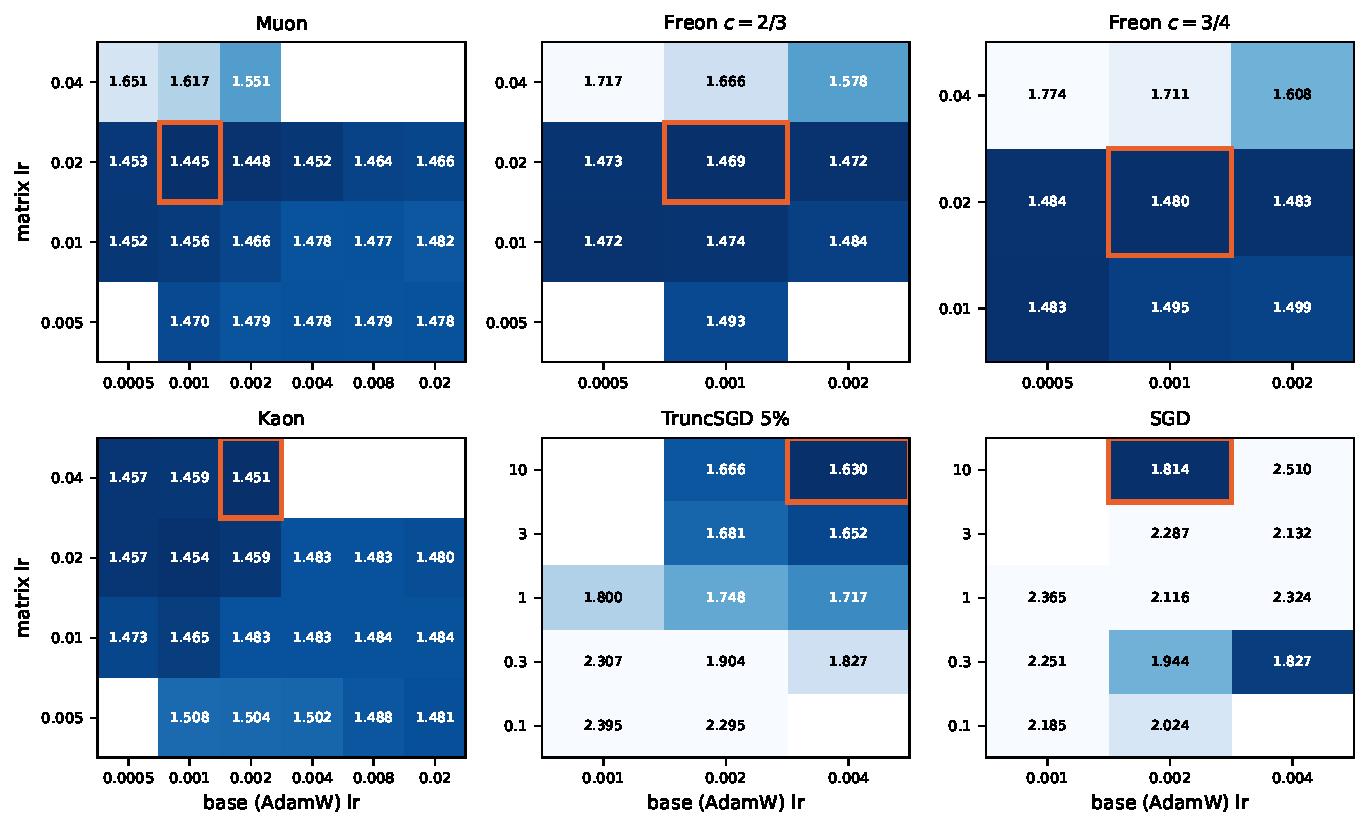
\includegraphics[width=\textwidth]{fig_h1_tune.pdf}
  \caption{Tuning grids (seed 42, 1500 steps): validation loss per (matrix lr, AdamW lr). The outlined cell is the setting used in Table~\ref{tab:h1main}. Blank cells were not run. Note the different matrix-lr ranges of the two SGD panels.}
  \label{fig:h1tune}
\end{figure}
All four flattening/random methods prefer $\eta_M=0.02$ (Kaon $0.04$) and a small $\eta_B$ ($\le2\times10^{-3}$); $\eta_M=0.04$ hurts Muon and both Freons badly, and Kaon is nearly flat at $\eta_M\in\{0.02,0.04\}$ ($1.451$--$1.459$), so its selected point ($\eta_M=0.04$, $\eta_B=2\times10^{-3}$) is not meaningfully better than its neighbours.
